\documentclass[11pt]{article}
\usepackage{ctex}
\usepackage[english]{babel}
\usepackage{blindtext}
\usepackage{nameref}
\usepackage{fancyhdr}
\usepackage{tabularx}
\usepackage{amsmath,amssymb,amsthm}
\usepackage{graphicx,float}
\usepackage{physics}
\usepackage{pgfplots}
\usepackage[a4paper, total={6in, 9in}]{geometry}
\usepackage{wrapfig}
\usepackage{scrextend}

\graphicspath{{../images/}}

\pagestyle{fancy}
\fancyhf{}
\fancyhf[HL]{Pre Senior Secondary test}
\fancyhf[CF]{\thepage}

\newcommand{\innerprod}[2]{\langle{#1},{#2}\rangle}
\newcommand{\id}{\mathtt{id}}

\newtheorem*{definition}{Definition}
\newtheorem*{theorem}{Theorem}
\newtheorem*{corollary}{Corollary}
\newtheorem*{lemma}{Lemma}
\newtheorem*{proposition}{Proposition}
\newtheorem*{remark}{Remark}
\newtheorem*{claim}{Claim}
\newtheorem*{example}{Example}
\newtheorem*{axiom}{Axiom}

\newenvironment{question}[1]{\par \textbf{Question #1.} \\ \begin{addmargin}[2em]{0cm}}{\hfill\textit{...end of question.}\end{addmargin}}

\begin{document}
    \thispagestyle{plain}

    \centering 

    \section*{Pre Senior Secondary test\\MATHEMATICS Compulsory Part\\Question-Answer Book}

    \raggedright

    \subsection*{Instructions}

    \begin{enumerate}
        \item This paper must be answered in English.
        \item Unless otherwise specified, all working must be clearly shown.
        \item Unless otherwise specified, numerical answers must be exact.
        \item This paper is for \textbf{internal use} only.
        \item All questions are collected from AL/CE/DSE past papers, reference site: https://www.dse.life/ppindex/m2/
    \end{enumerate}

    \newpage

    \section*{Number and algebra}

    \begin{question}{1}
        Let $i$ be some number satisfying the condition $i^2=-1$. I know it is strange, but we may call it the imaginary number. You will learn more about it in the future, for future I mean in S.4.

        Now, see $i$ as any algebraic expressions or variables as you have seen before. Just remember that $i^2=-1$ is applicable. Answer the following question.

        \begin{enumerate}
            \item Compute $(7+4i)-(3+24i)$.
            \item Compute $(6+8i)(6-8i)$.
            \item If $x^2=-4$, find $x$ in terms of $i$.
        \end{enumerate}
    \end{question}

    \hrulefill

        \hrulefill
            
        \hrulefill
        
        \hrulefill
        
        \hrulefill
        
        \hrulefill
        
        \hrulefill
        
        \hrulefill
        
        \hrulefill
        
        \hrulefill
        
        \hrulefill
        
        \hrulefill

        \hrulefill

        \hrulefill
            
        \hrulefill
        
        \hrulefill
        
        \hrulefill
        
        \hrulefill
        
        \hrulefill
        
        \hrulefill
        
        \hrulefill
        
        \hrulefill
        
        \hrulefill
        
        \hrulefill

        \hrulefill

        \hrulefill
            
        \hrulefill
        
        \hrulefill
        
        \hrulefill
        
        \hrulefill
        
        \hrulefill
        
        \hrulefill
        
        \hrulefill
        
        \hrulefill
        
        \hrulefill
        
        \hrulefill
            
        \hrulefill
        
        \hrulefill
        
        \hrulefill
        
        \hrulefill
        
        \hrulefill
        
        \hrulefill
        
        \hrulefill
        
        \hrulefill
        
        \hrulefill
        
        \hrulefill
        
        \hrulefill
        
        \hrulefill
        
        \hrulefill
        
        \hrulefill
        
        \hrulefill
        
        \hrulefill
        
        \hrulefill
        
        \hrulefill
        
        \hrulefill
        
        \hrulefill
        
        \hrulefill
        
        \hrulefill
        
        \hrulefill
        
        \hrulefill

    \pagebreak

    \begin{question}{2}
        Let's acknowledge the following two facts:\begin{theorem}
            If $x>0$, then $-x<0$.
        \end{theorem}\begin{theorem}
            If $x>0$ and $y>0$, then $xy>0$.
        \end{theorem}

        Using only the above facts, show the following:\begin{enumerate}
            \item If $x<0$ and $y>0$, then $xy<0$;
            \item If $x>0$ and $y<0$, then $xy<0$;
            \item If $x<0$ and $y<0$, then $xy>0$.
        \end{enumerate}
    \end{question}

    \hrulefill

        \hrulefill
            
        \hrulefill
        
        \hrulefill
        
        \hrulefill
        
        \hrulefill
        
        \hrulefill
        
        \hrulefill
        
        \hrulefill
        
        \hrulefill
        
        \hrulefill
        
        \hrulefill

        \hrulefill

        \hrulefill
            
        \hrulefill
        
        \hrulefill
        
        \hrulefill
        
        \hrulefill
        
        \hrulefill
        
        \hrulefill
        
        \hrulefill
        
        \hrulefill
        
        \hrulefill
        
        \hrulefill

        \hrulefill

        \hrulefill
            
        \hrulefill
        
        \hrulefill
        
        \hrulefill
        
        \hrulefill
        
        \hrulefill
        
        \hrulefill
        
        \hrulefill
        
        \hrulefill
        
        \hrulefill
        
        \hrulefill
            
        \hrulefill
        
        \hrulefill
        
        \hrulefill
        
        \hrulefill
        
        \hrulefill
        
        \hrulefill
        
        \hrulefill
        
        \hrulefill
        
        \hrulefill
        
        \hrulefill
        
        \hrulefill
        
        \hrulefill
        
        \hrulefill
        
        \hrulefill
        
        \hrulefill
        
        \hrulefill
        
        \hrulefill
        
        \hrulefill
        
        \hrulefill
        
        \hrulefill
        
        \hrulefill
        
        \hrulefill
        
        \hrulefill
        
        \hrulefill
        
        \hrulefill
        
        \hrulefill

    \pagebreak

    \section*{Measurement}

    \begin{question}{1}
        We know that we have to use a ruler to measure lengths of different objects. Assume that we have a ruler of length 20cm with 198 evenly distributed lines on it throughout the ruler.

        Some researchers find that factories might make a small error on the length of a ruler, which is at most 0.01 cm.

        Find the relative error of the measurement by this kind of ruler, if the object is measured as 20 cm.
    \end{question}

    \hrulefill

        \hrulefill
            
        \hrulefill
        
        \hrulefill
        
        \hrulefill
        
        \hrulefill
        
        \hrulefill
        
        \hrulefill
        
        \hrulefill
        
        \hrulefill
        
        \hrulefill
        
        \hrulefill
        
        \hrulefill
        
        \hrulefill
        
        \hrulefill
        
        \hrulefill
        
        \hrulefill
        
        \hrulefill
        
        \hrulefill
        
        \hrulefill
        
        \hrulefill
        
        \hrulefill
        
        \hrulefill
        
        \hrulefill
        
        \hrulefill
        
        \hrulefill
        
        \hrulefill
        
        \hrulefill

        \hrulefill

        \hrulefill
            
        \hrulefill
        
        \hrulefill
        
        \hrulefill
        
        \hrulefill
        
        \hrulefill
        
        \hrulefill
        
        \hrulefill
        
        \hrulefill
        
        \hrulefill
        
        \hrulefill

        \hrulefill

        \hrulefill
            
        \hrulefill
        
        \hrulefill
        
        \hrulefill
        
        \hrulefill
        
        \hrulefill
        
        \hrulefill
        
        \hrulefill
        
        \hrulefill
        
        \hrulefill
        
        \hrulefill
            
        \hrulefill
        
        \hrulefill
        
        \hrulefill
        
        \hrulefill
        
        \hrulefill
        
        \hrulefill
        
        \hrulefill
        
        \hrulefill
        
        \hrulefill
        
        \hrulefill

    \pagebreak

    \begin{question}{2}
        Refer to the following figures:

        \begin{figure}[H]
            \centering
            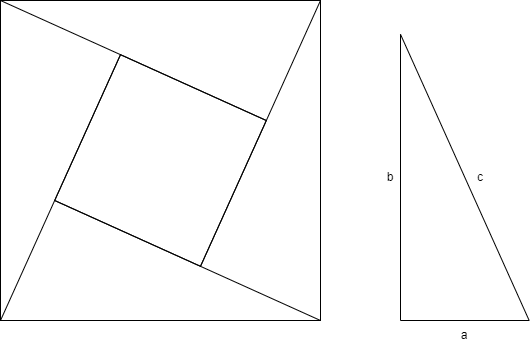
\includegraphics[scale=0.6]{pythagoras.png}
        \end{figure}

        Given a big square of side length $c$ and a small square of side length $a$, and every lines in the left figures are straight lines.

        \begin{enumerate}
            \item Ignoring the left figure, prove that every triangles in the right figure are all right-angled triangles. Prove also that all 4 triangles are identical (i.e. they are all congruent to each other).[You should name the vertices by yourself when needed.]
            \item Consider the right figure as details of each triangle, prove the Pythagoras theorem: $$a^2+b^2=c^2$$
            \item Prove from above result, that \begin{enumerate}
                \item $\sin^2{\theta}+\cos^2{\theta}=1$;
                \item $\tan^2{\theta}+1=\dfrac{1}{\cos^2{\theta}}$.
            \end{enumerate}
        \end{enumerate}
    \end{question}

    \hrulefill

        \hrulefill
            
        \hrulefill
        
        \hrulefill
        
        \hrulefill
        
        \hrulefill
        
        \hrulefill
        
        \hrulefill
        
        \hrulefill
        
        \hrulefill
        
        \hrulefill
        
        \hrulefill
        
        \hrulefill
        
        \hrulefill
        
        \hrulefill
        
        \hrulefill
        
        \hrulefill
        
        \hrulefill
        
        \hrulefill
        
        \hrulefill
        
        \hrulefill
        
        \hrulefill
        
        \hrulefill
        
        \hrulefill
        
        \hrulefill
        
        \hrulefill
        
        \hrulefill
        
        \hrulefill
        
        \hrulefill
        
        \hrulefill
        
        \hrulefill
        
        \hrulefill
        
        \hrulefill
        
        \hrulefill
        
        \hrulefill
        
        \hrulefill
        
        \hrulefill
        
        \hrulefill
        
        \hrulefill
        
        \hrulefill
        
        \hrulefill
        
        \hrulefill
        
        \hrulefill
        
        \hrulefill

        \hrulefill

        \hrulefill
            
        \hrulefill
        
        \hrulefill
        
        \hrulefill
        
        \hrulefill
        
        \hrulefill
        
        \hrulefill
        
        \hrulefill
        
        \hrulefill
        
        \hrulefill
        
        \hrulefill

        \hrulefill

        \hrulefill
            
        \hrulefill
        
        \hrulefill
        
        \hrulefill
        
        \hrulefill
        
        \hrulefill
        
        \hrulefill
        
        \hrulefill
        
        \hrulefill
        
        \hrulefill
        
        \hrulefill
            
        \hrulefill
        
        \hrulefill
        
        \hrulefill
        
        \hrulefill
        
        \hrulefill
        
        \hrulefill
        
        \hrulefill
        
        \hrulefill
        
        \hrulefill
        
        \hrulefill

    \pagebreak

    \section*{Data Handling}

    \begin{question}{1}
        Given 3 fair dice.\begin{enumerate}
            \item If luckily, every sums from these 3 dice is obtained once. (We mean the sum from 3 dice by getting the result of each dice by rolling them in once, and adding the results up to obtain a sum.) Find the mean and median of the distribution.
            \item Find the probability of getting the median sum.
        \end{enumerate}
    \end{question}

    \hrulefill

        \hrulefill
            
        \hrulefill
        
        \hrulefill
        
        \hrulefill
        
        \hrulefill
        
        \hrulefill
        
        \hrulefill
        
        \hrulefill
        
        \hrulefill
        
        \hrulefill
        
        \hrulefill

        \hrulefill

        \hrulefill
            
        \hrulefill
        
        \hrulefill
        
        \hrulefill
        
        \hrulefill
        
        \hrulefill
        
        \hrulefill
        
        \hrulefill
        
        \hrulefill
        
        \hrulefill
        
        \hrulefill
        
        \hrulefill
        
        \hrulefill
        
        \hrulefill
        
        \hrulefill
        
        \hrulefill
        
        \hrulefill
        
        \hrulefill
        
        \hrulefill
        
        \hrulefill
        
        \hrulefill
        
        \hrulefill
        
        \hrulefill
        
        \hrulefill
        
        \hrulefill
        
        \hrulefill
        
        \hrulefill

        \hrulefill

        \hrulefill
            
        \hrulefill
        
        \hrulefill
        
        \hrulefill
        
        \hrulefill
        
        \hrulefill
        
        \hrulefill
        
        \hrulefill
        
        \hrulefill
        
        \hrulefill
        
        \hrulefill
            
        \hrulefill
        
        \hrulefill
        
        \hrulefill
        
        \hrulefill
        
        \hrulefill
        
        \hrulefill
        
        \hrulefill
        
        \hrulefill
        
        \hrulefill
        
        \hrulefill

    \pagebreak

\end{document}